\documentclass[11pt,a4paper]{article}

\usepackage[english]{babel}
\usepackage[utf8]{inputenc}
\usepackage{amsmath}
\usepackage{graphicx}
\usepackage[colorinlistoftodos]{todonotes}
\usepackage{pdfpages}

\begin{document}

\begin{titlepage}

\newcommand{\HRule}{\rule{\linewidth}{0.5mm}} 

\center 

\textsc{\LARGE KING's COLLEGE LONDON}\\[1.5cm] 
\textsc{\Large 7CCSMGPR Group Project Module}\\[0.5cm] 
\textsc{\large TEAM KINGSMEN}\\[0.5cm] 

\HRule \\[0.4cm]
{ \huge \bfseries TRAFFIC SIMULATOR}\\[0.4cm] 
\HRule \\[1.5cm]

\begin{minipage}{0.4\textwidth}
\begin{flushleft} \large
\emph{Authors:}\\
Vikram Prabhu \\
Vijay Kumar Badatala \\
Praveen Allu \\
Nuruzzaman Shahin \\
Bhabishya Shrestha \\
\end{flushleft}
\end{minipage}
~
\begin{minipage}{0.4\textwidth}
\begin{flushright} \large
\emph{Supervisors:} \\
Dr. Laurence Tratt \\
Dr. Elizabeth Black
\end{flushright}
\end{minipage}\\[4cm]

{\large March 28, 2016}\\[6cm]

\end{titlepage}

\tableofcontents

\newpage

\section{INTRODUCTION}

Majority of road accidents that happen in today’s world are because of human error. Around 1.3 million people die in road accidents every year which on an average turns out to be around 3287 deaths a day. To minimize these road accidents, we need a program like a Traffic Management System. Traffic Management Systems can improve flow of vehicles and also improve the safety of people. It would be best to develop a Traffic Simulation Software that can take care of the above factors. In this way, transportation systems can be properly mathematically modelled by the use of a computer software which can help plan and design a better and safer traffic system.


\section{OVERVIEW}

The aim of this ‘7CCSMGPR Group Project’ Module is to give students the experience in developing a rather complex software application whilst helping them to face challenges during the development and also the challenges involved in working in a team/group. The aim is to build a traffic simulation engine that will help to improve the flow of traffic. The simulation engine would also help in giving way to emergency vehicles even during blocked roads so that these vehicles are able to reach their destination in times of emergencies or natural calamities. \newline
Our approach in tackling this problem started with the requirements elicitation and will most probably be followed by designing the architecture of the software application. 


\section{STRATEGY}

While going through various approaches/strategies, we finally decided to adopt Object Oriented Programming. We decided to split into two teams, the ‘User Interface Team’ and the ‘Simulation Team’. We adopted the Agile Methodology which helped both the teams at each stage as the life cycle of the development of the software advances. The latter or final stages of the project mostly included software testing, bug fixing and final documentation.

\section{PROJECT AIM}

The aim of this project was to develop a traffic simulation software that would aid in testing various traffic management system strategies. This software would allow users to use various parameters and generate any kind of road network. Users are also able to select different vehicle types, density of the traffic, synchronization of the traffic lights, behaviour of the drivers etc. The software would generally be able to simulate vehicles such as ‘Light Vehicles’, ‘Heavy Vehicles’ and a special category of vehicles such as ‘Emergency Vehicles’. The simulation software should also be able to show for different driver behaviours such as ‘Normal’ Driver and ‘Over-Speeding’ or ‘Dangerous’ Driver. It also accounts for weather conditions such as Sunny and Snowy.


\section{PROJECT OUTCOME}

Our software accomplishes the goal by allowing the user to configure traffic pattern options contributed by different vehicle types such as cars, emergency vehicles, the traffic density for various vehicle types, the traffic lights synchronisation, driver behaviour, climatic conditions.


\section{LITERATURE REVIEW}

There are various techniques utilized for movement simulation software underneath we give a brief outline of some of them that are more pertinent to our methodology. 

\subsection{TRAFFIC SIMULATION USING AGENT BASED MODELLING}

Agent Based Model is a very effective method of building the simulation for real life software project. The model comprises of entities called agents that have their individual behaviour and the decision-making heuristics of the environment its in. Agent based models cannot be estimated in differential equations which is why the agents should have an ability to adapt to the environment its in and interact with the same.
Agent based models are used in the following situations:

\begin{itemize}
\item When the granularities of the objects are not defined.
\item When it is important that all the agents have dynamic relationships with all the other agents, and the agent relationships are made and dissolved.
\item When the complex communication topology can cause problems to the entire main system.
\item When some of the defined mathematical equations eliminate the most important aspect of the individual behaviour which can cause damage the entire main system.
\end{itemize}
Agent based traffic models also include more measurable behaviour of the drivers for instance, each and every agent will have their individual behaviour which can affect the vision, speed and distance to keep the other vehicles from colliding. 





\subsection{INTRODUCTION TO TRAFFIC SIMULATION}

Simulation is a successful tool utilized for imitating and analysing a wide assortment of complex issues, hard to think about by different implies that may be excessively costly or risky. Traffic can be seen as an intricate framework along these lines so simulation is a suitable instrument to analyse movement frameworks. Traffic Simulation is the best in class technique used to survey and assess transport plans for decreasing congestion. As opposed to implementing a plan without knowing whether the result will be a win, the plan can be executed in a simulation to decide its viability.\newline
Simulations can be classified as continuous or discrete. Continuous models take the type of mathematical equation utilizing variables that compare to genuine qualities. By comprehending the mathematical equations, the condition of the model at any given point in the simulation can be figured. Discrete simulations show the reality by demonstrating the condition of the framework and its state changes after time or occasions have passed. There are two sorts of discrete simulations: discrete time models and discrete even models. Discrete time models (time-cut) are those that split the simulations into settled time interims. At every interim, the condition of the model is upgraded utilizing capacities that portray the connections. Discrete event models (event arranged) are those which keep up a line of events booked to happen all together of time, every event speaking to the change of condition of a component in the model. The test system forms the event all together, and every one can modify the event line.


\subsection{MICROSCOPIC SIMULATION}

Traffic Simulators can be macroscopic or microscopic relying upon the level of point of interest required. Naturally visible test systems show the stream of traffic utilizing abnormal state numerical models regularly got from fluid dynamics, in this manner they are consistent simulations. They treat each vehicle the same, and use data and yield variables, for example, velocity, stream and density. These traffic simulations can't separate between individual vehicles, and typically don't cater for various vehicle sorts. They do not have the capacity to model complex roadways, itemised movement control highlights or distinctive driver practices. Macroscopic Simulators are most helpful for the recreation of wide-range movement frameworks, which don't require detailed modelling, for example, motorway systems and interregional street systems. This methodology is not extremely reasonable on the grounds that, in actuality, there are a wide range of sorts of vehicle driven by various people who have their own styles and practices. Notwithstanding, it is quick and can be valuable and precise, however is not suited to urban models.\newline 
Microscopic Simulators model individual substances independently at an abnormal state of point of interest, and are classed as discrete simulations. Every vehicle is followed as it associates with different vehicles and nature. Interactions are normally represented via auto taking after and path evolving rationale. Principles and regulations are characterized to control what should and can't be possible in the recreation, for instance speed limits, privileges of way, vehicle pace and quickening. Traffic flow details generally connected with naturally visible simulations are the developing properties of the minute simulations. Microscopic simulators can demonstrate traffic flow more reasonably than microscopic simulators because of the additional subtle element included displaying vehicles exclusively. Microscopic test systems are generally used to assess new activity control and administration innovations and also performing investigation of existing traffic operations.


\subsection{AGENT- BASED MODELLING}

Simulation can be executed utilising multi-agent frameworks; this is known as multi-agent simulation or agent based modelling. The agent worldview maps conveniently onto numerous modelling situations since every individual in the situation can be specifically spoken to as a specialists. Behaviours can be modified into the specialists so people act similarly as the element they are demonstrating. A fascinating point is that people are given basic practices, and when numerous agents are simulated as a gathering, practices regularly rise that were not unequivocally customised into the specialists; these are known as rising phenomenon.\newline 
This proposes multi-agent simulation can be a excellent prototyping tool for creating and refining models. Since it can permit parameters of the people and the earth to be fluctuated effortlessly, it is conceivable to explore different avenues regarding numerous choices and increase results in real-time. 


\subsection{DIFFERENCES TO OBJECT- ORIENTED PROGRAMMING}

To help understanding, the agent- oriented methodology could be considered as an augmentation to the item arranged (OO) approach. Objects are processing substances that epitomise some state, have strategies to change their state, and convey by passing messages. Objects in this manner have some type of control over their state, yet they don't have control over their conduct. Agents are considered to have control over their conduct, implying that every agent has its own particular string of control and can perform activities at whatever point it picks without being followed up on by some other substance. Despite the fact that it is workable for all items to have their own string of control, it is not fundamental to the OO idea.\newline 
Agents additionally display adaptable conduct, which is not part of the OO worldview. This implies they are fit for responsive, proactive and social conduct. Receptive means they can see and react to changes in their surroundings, proactive means they can take the activity to accomplish their objectives, and social means they can connect with different agents to satisfy their goals.
 



\section{TRAFFIC SIMULATION}
 
\subsection{SCENARIO FOR SIMULATION}

Simulators supporting a motorway situation concentrate on multiple-lane fast motorways. A significant part of the many-sided quality required for a city domain does not should be displayed, and the simulation can concentrate on vehicle conduct and communication. Motorway situations can be simulated precisely by both macroscopic and microscopic simulators. The principle features of a microscopic motorway simulators are car following and lane changing perspectives. Junctions are once in a while demonstrated, permitting passage/exit rate to be fluctuated to test the productivity of the motorway under differing movement load.


\subsection{ISSUES IN MODELLING}

Defining the model is one of the main phases in building a traffic simulator. This includes choosing how to show objects (e.g. vehicles, traffic lights and people) in the simulation and what parameters every object will require. It likewise includes deciding how to represent the environment (e.g. street, paths and crossing points), and the impacts it has on the other objects.


\subsection{MODELLING THE VEHICLES}

In a simulation, vehicles and drivers would undoubtedly be demonstrated as one entity. In any case, in this real world they clearly are not, so when settling on the best way to model them it bodes well to take a look at each in turn. Displaying a vehicle is entirely straightforward; a couple of parameters can portray its features and conduct: maximum speed, maximum acceleration and deceleration. Acceleration is particularly critical as it influences the rate of queue release. Measurements are regularly actualised, empowering trucks and transports to be recognised from cars. Amid simulation, current position and heading in nature are required to monitor the present state. Different points of interest are not typically required in light of the fact that they add to the many-sided quality without enhancing authenticity, however a few test systems give detailed physics or engine models; these are valuable when researching outflows or the itemised impacts of effect.


\subsection{MODELLING THE DRIVERS}

Decision drivers need to make can be split into macro and micro objectives. Macro objectives are the destination and course taken, while micro objectives include choices at every purpose of time in light of a legitimate concern for accomplishing the macro objective. The macro objective includes day by day arranging and course generation usefulness, frequently enter from O-D information. Micro objectives are choices including controlling the vehicle, for example, desired speed, overtaking and turning. Drivers all have distinctive driving styles, which are represented by their individual attributes, for example, forcefulness, certainty and driving knowledge. Driving styles are frequently approximated utilising parameters for essential behavioural components and after that these qualities are utilised as a feature of the thinking procedure to work out the choice a driver would take at any moment. Illustrations of these parameters are: 
\begin{itemize}
\item Favoured speed: the velocity the driver likes to keep up on an empty street. 
\item Favoured rate of acceleration: which is not usually the vehicle's maximum rate, but rather a rate impacted by a driver's forcefulness and longing for comfort among different attributes. 
\item Favoured rate of deceleration: which is similar to acceleration. 
\item Gap Acceptance: which is the distance a driver likes to keep between himself and the vehicle ahead of him.
\end{itemize}
These parameters can show a considerable measure of driver attributes. A reckless driver would have a high favoured speed, a high favoured rate of acceleration and deceleration, and a little gap acceptance. A cautious driver would be much the inverse. Many simulators consolidate these parameters, and exhibit sensible driving conduct. To change over these parameters into actions, a thinking process must be assessed at every phase of the simulation.



\subsection{ENVIRONMENT MODELLING}

In traffic simulation, environment in which vehicles drive is a street network which is comprised of connection sections, hubs (intersections and crossing points) and control highlights which are normally part of the hub. Every connection can have one or more paths, and might work in one or both directions. Hubs can be separated into the accompanying essential sorts: uncontrolled non-priority intersections, priority intersections, roundabouts, signal controlled intersections and grade partition intersections. Extraordinary instances of connection exist, for example, merges where two paths must converge into one, wanders where one path parts into two and weaving segments where a diverge nearly follows a merge. Cases of other control components are traffic calming plans and people intersections.\newline 
Models typically represent the network as a gathering of connections joined by hubs. Hubs have properties, for example, area (e.g. co-ordinates) and sort of hub. Joins have properties, for example, length, number of paths, speed limit, and so on. For street networks that are not independent, sources and sinks are made as positions in the system where vehicles arrive and leave individually. Sources have parameters that decide the rate of entry of vehicles into the network, and sinks dependably uproot vehicles that go to them.



\subsection{SIMULATION ISSUES}

Models of vehicles, drivers and the environment are of no utilisation unless they can be controlled amid simulation. Simulation includes utilising behavioural guidelines to change the model after some time. This includes moving every vehicle in view of its parameters and its driver's choices. To mimic a single car on a long straight street is fairly simple as the vehicle would simply accelerate to the driver's favoured speed. It turns out to be progressively complex as different vehicles, more paths, and more streets are presented; to manage these, vehicle following and lane changing models are utilised.

\subsubsection{\textbf{Vehicle Following}}

Vehicle following models are those that endeavour to portray how a vehicle acts in standard conditions. These models are called such on the grounds that they concentrate fundamentally on the relationship between the current car and the one ahead of it. Numerous vehicle following models are discussed, and a number of these depend on anti-collision ideas.\newline 
One understood model of this sort is the Gipps model, created in 1981. It expects that a vehicle dependably intends to have the capacity to stop securely if the one ahead of it performs an immediate stop. It ascertains the new speed of the accompanying vehicle utilising the flow speed of both vehicles, the accompanying driver's desired pace, maximum acceleration and deceleration, and the distance between vehicles. It ascertains two conceivable qualities for rate; one in light of the driver's sought speed restricted by vehicle execution, and one in view of security, i.e. the speed that should be taken to guarantee there is no collision. It then chooses the minimum of these conceivable speeds to use in the simulation, which guarantees both impediments are applied.\newline
Another class of models are known as psycho-physical vehicle following models. These models endeavour to catch both physical and human segments of vehicle control. They do this by keeping up a vehicle state, where the current state is resolved through contrasts in speed and the distance to the main vehicle. Every state has an alternate technique for figuring the acceleration of the vehicle, and upon a state change, the new acceleration is ascertained once and is then consistent until the next change of state. Since the acceleration is not figured at every time venture in the simulation, it has been demonstrated that the event arranged time advance strategy is extremely effective for this model. State changes can be resolved and recorded in a line so they can be handled all together.


\subsubsection{\textbf{Lane Changing}}

Lane changing models are those that depict when and how vehicles move to another lane on a multi-lane street, for example, a motorway. The behaviour of every vehicle relies on the vehicles around it, and every vehicle needs to settle on choices taking into account its information of the environment. Path changing models have been studied to a comparable extent as vehicle following models, and a few vital models have been conceived.\newline
Lane change issues rise up from street rules, for instance in the U.K. passing is ordinarily just permitted on the right and vehicles ought to attempt to keep on the left lane. Driver qualities can likewise have influence, since a few drivers like to stay in the same lane regardless of the fact that moving to another lane would bring about a higher speed, and a few drivers want to stay in outer lanes regardless of the fact that there is space in the inner lanes.



\section{REQUIREMENTS AND DESIGN}

\subsection{INITIAL REQUIREMENTS, GOALS AND PLAN}

The various approaches that could be used for the development of the simulation engine in NetLogo were considered and assessed.

\subsubsection{NetLogo}

NetLogo is an agent based modelling environment intended for simulating complex regular and social phenomena. It is written in Java and is in this manner cross-stage, it is freeware, and has a huge benevolent client bunch. It empowers the client to model any number of agents in a variable-size environment utilising a basic programming language got from Logo. It is intended for use by students and analysts to investigate the conduct of customised agents under differing conditions. It takes after the theory of 'low threshold, no ceiling', implying that new clients ought to think that its simple to begin, however advanced clients ought not think that its restricting. NetLogo accompanies broad documentation, tutorials, and more than 300 example models that exhibit all parts of the device. Models can be saved as Java Applets and keep running on website pages by any client with the Java Virtual Machine installed. It is conceivable to see the present condition of the environment and specialists in 2D or 3D, and operators can be given any vector shape to show their sort. Commands can be as techniques that are called by buttons on the interface, or entered straightforwardly in the summon console on the fundamental board. Its logo-esque language is very common, permitting code to be anything but difficult to read, write and understand.\newline 
NetLogo has a well designed graphical interface and interface manufacturer in one that permits the novice and expert alike to run, change and create models effortlessly. It gives numerous implicit gadgets to change simulation parameters at runtime, including sliders, catches, and drop-down menus, and permits yield as charts and variable screens. Simulation time is measured in discrete 'ticks', and simulation pace can be balanced by a slider over the presentation. It can give deterministic simulation if the random seed is set before the simulation is run.\newline
Since all the given requirements were generic, we revisited and re-defined the requirements to generate a formal requirements report.

\subsection{SOFTWARE DESIGN}

\subsubsection{\textbf{Interaction Diagrams}}

Sequence Diagrams are a sort of interaction diagrams that demonstrate the stream of messages through a framework as a specific function is being executed. Below are two sequence diagrams portraying the sequence occurring during a simulation tests. It portrays a single time-step, and amid typical use, these sequences could be rehashed for the simulation duration. \newpage

\begin{figure}[!ht]
\centering
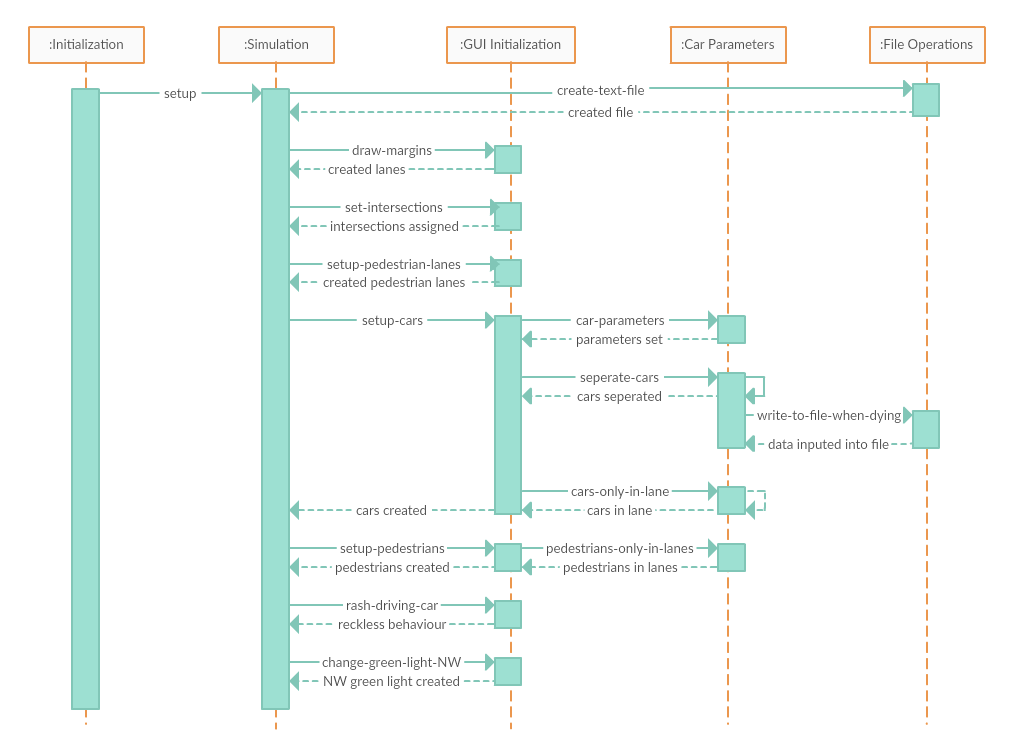
\includegraphics[width=0.8\textwidth]{sequenceDiagram1.png}
\caption{\label{fig:sd1}Sequence Diagram for "setup" procedure.}
\end{figure}

\begin{figure}[!ht]
\centering
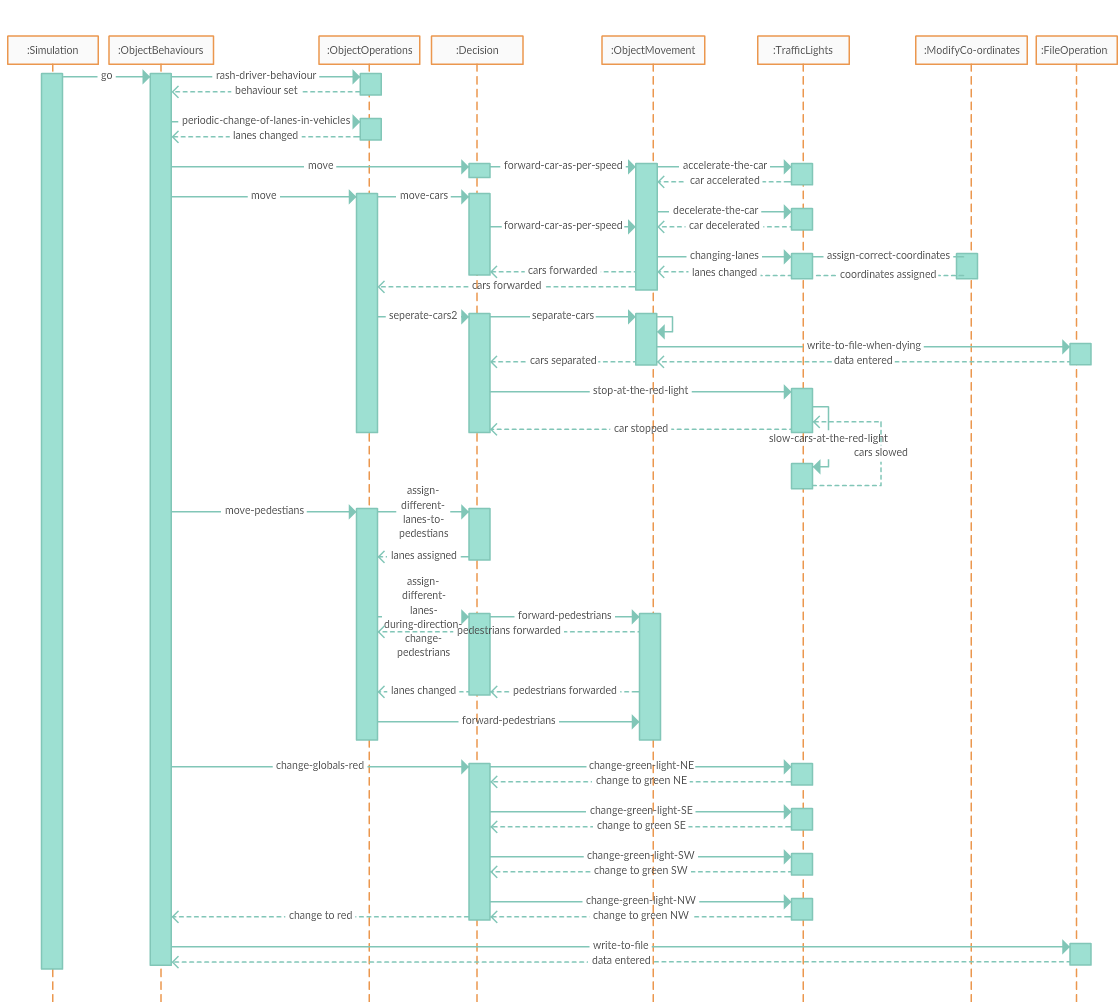
\includegraphics[width=0.8\textwidth]{sequenceDiagram2.png}
\caption{\label{fig:sd2}Sequence Diagram for "go" procedure.}
\end{figure}

\newpage
\subsubsection{\textbf{Class Diagram}}

NetLogo gives numerous inbuilt turtle and patch variables, just the ones which are significant to the project are appeared on the chart. All properties and system are open since any agent can query one other, in this way zero visibility will be shown. Despite the fact that NetLogo does not give an object - oriented environment, conceptually the framework will be composed using OO procedures. Although every system could be called by any agent, every procedure is particular to one sort or type of agent. In this diagram, blue classes are those given by NetLogo, and white show those components included for this software.

\begin{figure}[!ht]
\centering
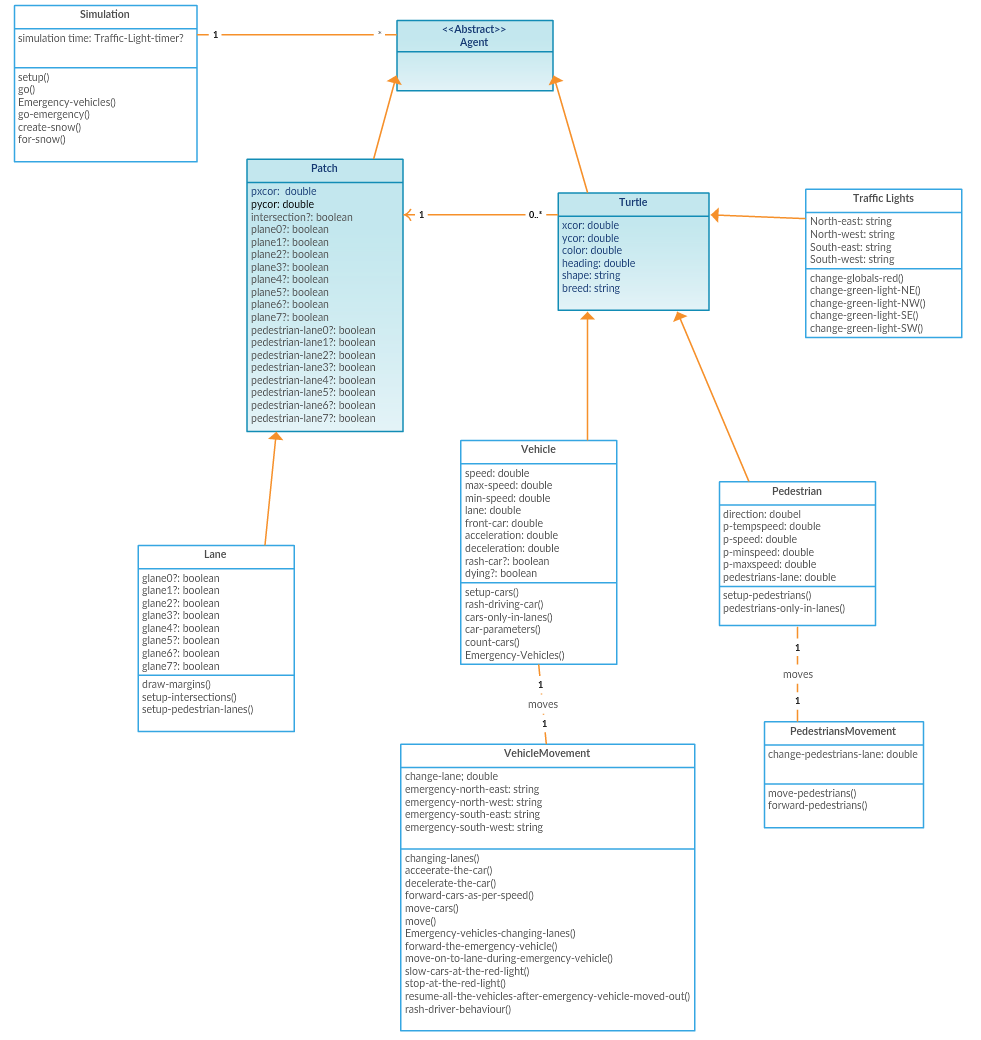
\includegraphics[width=0.7\textwidth]{classDiagram1.png}
\caption{\label{fig:cd1}Class Diagram.}
\end{figure}

\section{SOFTWARE DEVELOPMENT, TESTING AND DOCUMENTATION}

We adopted the Agile Methodology of software development. As mentioned earlier, the group was divided into two teams namely User Interface Team which is the Front End Team and the Simulation Team which is the Back End Team. Each team was assigned major tasks and other sub tasks so that the whole group worked in parallel collaboration. Regular meetings were held for further task identifications, task allocations, development, testing etc.\newline
For software design and architecture, we approached the problem using the following architectural methodologies and patterns:
\begin{itemize}
\item We decomposed the problem and defined the use case. 
\item We identified the various components in the environment, their interactions and dependencies with UML. Also we identified the attributes and methods of each sub component using ArgoUML. 
\item We grouped the related components into different controllers and developed the contracts of the interface with the method signatures for the interactions between the User Interface and Simulation Engine.
\end{itemize}

\section{PROJECT PLAN}

As shown in the Gantt Chart below, we carefully segregated the time allotted to complete the development of the software project. We gave around 2-3 weeks to the planning phase. In this phase we learnt a new simulation software called NetLogo as most of the group members didn’t have prior programming experience. The second and undoubtedly the longest phase was that of Development Phase. Each team segregated their tasks in sprints of around 7 days in which development, unit, functional testing, error testing and integration of units were involved. This was then followed by the testing phase done in the final week in which we carried out the performance testing. The Documentation or Report Generation was carried out as and when we were developing the system.

\begin{figure}[!ht]
\centering
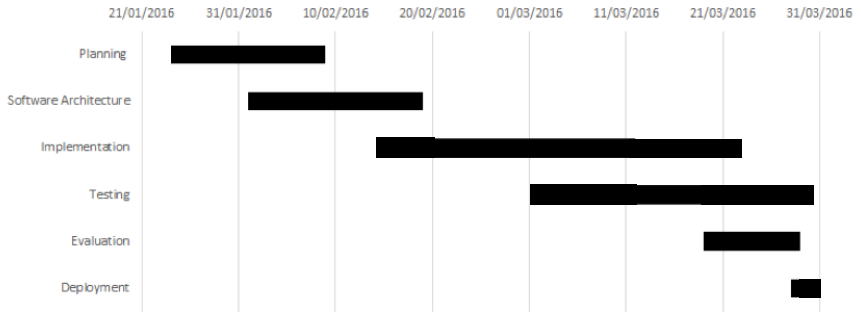
\includegraphics[width=0.9\textwidth]{GC.PNG}
\caption{\label{fig:gc}Gantt Chart.}
\end{figure}

Main Aims:

\begin{enumerate}
\item Selection of different traffic light cycles, various types of drivers, types of vehicles etc.
\item Implementation of driver behaviour.
\item Reports to be generated for various traffic management strategies.
\end{enumerate}


\section{USER INTERFACE (FRONT-END) DESIGN AND IMPLEMENTATION}

The User Interface Team was responsible for the design of the system.

\subsection{\textbf{Design of Lanes}}

We designed a 4-road junction with 2 lane roads, where we grouped certain number of patches into one lane of a road. For example: Patches with x co-ordinate less than or equals to -3 and y co-ordinate equals to 3 constitute lane 0.

\begin{figure}[!ht]
\centering
\includegraphics[width=0.7\textwidth]{Design_of_Lanes.png}
\caption{\label{fig:dol}Design of Lanes.}
\end{figure}
                                    
\subsection{\textbf{Design of Traffic Lights}}

We used patches to generate traffic signals which have been highlighted in the below figure. The patches circled in blue are the ‘Red’ traffic lights which signals the vehicles to halt. The patch circled in red is the ‘Green’ traffic light which signals the vehicle to proceed further.

\newpage
\begin{figure}[!ht]
\centering
\includegraphics[width=0.7\textwidth]{Design_of_Traffic_Signalling_System.png}
\caption{\label{fig:dotss}Design of Traffic Signalling System.}
\end{figure}
                                    
\subsection{\textbf{Generation of Pedestrian System}}

We used turtles and patches to design the complete Pedestrian System, where a number of patches are grouped together to design a pedestrian lane which is in black colour as shown in the figure below. Whereas, the turtles are used to show the pedestrians on the pedestrian lane. For example: The turtles circled in yellow are some of the pedestrians.\newline
We have used different colours for different pedestrians so that we can easily differentiate between the pedestrians who are going in different directions.

\begin{figure}[!ht]
\centering
\includegraphics[width=0.7\textwidth]{Pedestrian_System_Design.png}
\caption{\label{fig:psd}Pedestrian System Design.}
\end{figure}
                                    
\subsection{\textbf{Generation of Cars}}

We used different turtles to show the various cars on the lanes.

\begin{figure}[!ht]
\centering
\includegraphics[width=0.7\textwidth]{Generation_of_Cars.png}
\caption{\label{fig:goc}Generation of Cars.}
\end{figure}
In order to identify the Emergency Vehicles, we have designed the emergency vehicles as highlighted below. We can also distinguish the Emergency Vehicles with the unique siren given.

\begin{figure}[!ht]
\centering
\includegraphics[width=0.7\textwidth]{Emergency_Vehicle.png}
\caption{\label{fig:ev}Emergency Vehicles.}
\end{figure}
                                   
\subsection{\textbf{Driver Behaviour}}

We have distinguished the driver behaviour in 2 ways namely:
\begin{itemize}
\item Cautious or Normal Driver
\item Over-speeding or Dangerous Driver
\end{itemize}
The Cautious Driver is a driver who drives at a regulated speed. On a general basis we have considered every normal driver as cautious by nature. For example: The cautious driver is highlighted in the figure below.

\begin{figure}[!ht]
\centering
\includegraphics[width=0.7\textwidth]{Cautious_Driver.png}
\caption{\label{fig:cd}Cautious or Normal Driver.}
\end{figure}

The Dangerous driver is a driver who always over-speeds while driving and always tries to overtake the other vehicles rashly. For example: The Dangerous Driver is highlighted in red colour by default as shown in the figure below.

\begin{figure}[!ht]
\centering
\includegraphics[width=0.7\textwidth]{Reckless_Driver.png}
\caption{\label{fig:rd}Over-speeding or Dangerous Driver.}
\end{figure}

\subsection{\textbf{Weather Conditions}}

We have considered 2 different weather conditions:
\begin{itemize}
\item Normal Condition
\item Snowy Condition
\end{itemize}
In Normal condition we have considered the drivers drive the cars at a regular speed without any precautions.\newline 
In Snowy Condition we have considered the drivers drive the car at a relatively slower speed when compared to normal conditions due to the difficulty of driving the cars in the snowy weather.

\begin{figure}[!ht]
\centering
\includegraphics[width=0.7\textwidth]{Snowy_Weather_Conditions.png}
\caption{\label{fig:swc}Snowy Weather Condition.}
\end{figure}

                                    
\section{SIMULATION (BACK-END IMPLEMENTATION)}


\subsection{PATCHES AND TURTLES IN NETLOGO}

\begin{itemize}
\item NetLogo teaches programming concepts using agents in the form of turtles, patches, links and observer.  
\item NetLogo allows exploration by modifying switches, sliders, choosers, inputs, and other interface elements
\item In NetLogo, patches are agents with a fixed location, always exist and are arranged as a grid. Turtles are agents that are able to move. They have implicit access to variables of the patch they are on.
\item NetLogo world has x-axis and y-axis with origin at (0,0) [ origin can be changed by the user ]. Each co-ordinate corresponds to one patch. Therefore each patch will have a dedicated x-cor and y-cor.
\end{itemize}


\subsection{IMPORTANT PROCEDURES USED IN SIMULATION (BACK-END IMPLEMENTATION)}

NetLogo, even though it implements agent based modelling, conceptually object oriented approach is used to design the system. We don’t have any concept of classes in this simulator but we do program procedures to attain some functionalities and these procedures can be called by any agent.\newline
In general, we design procedures corresponding to a particular breed or agent of only one type. In our project we used four breeds namely cars, ambulances, pedestrians and water. They are initiated by the following lines of code in the project: 
                breed[cars car]
                breed[pedestrians pedestrian]
                breed[ambulances ambulance]
                breed[water]

The two main methods in our project which call some of the important procedures are: 
\begin{enumerate}
\item setup()
\item go()
\end{enumerate}
NetLogo simulator has two important tabs: 
\begin{itemize}
\item Interface
\item Code
\end{itemize}
Interface – In this tab one can actually see the simulation scenarios and can select different behaviors using sliders, choosers, buttons, etc.\newline
Code – In this tab documentation of the code is done. Depending upon the way we code in this tab, interface tab will change the NetLogo world accordingly.
The user interface tab of our project looks as follows: 

\begin{figure}[!ht]
\centering
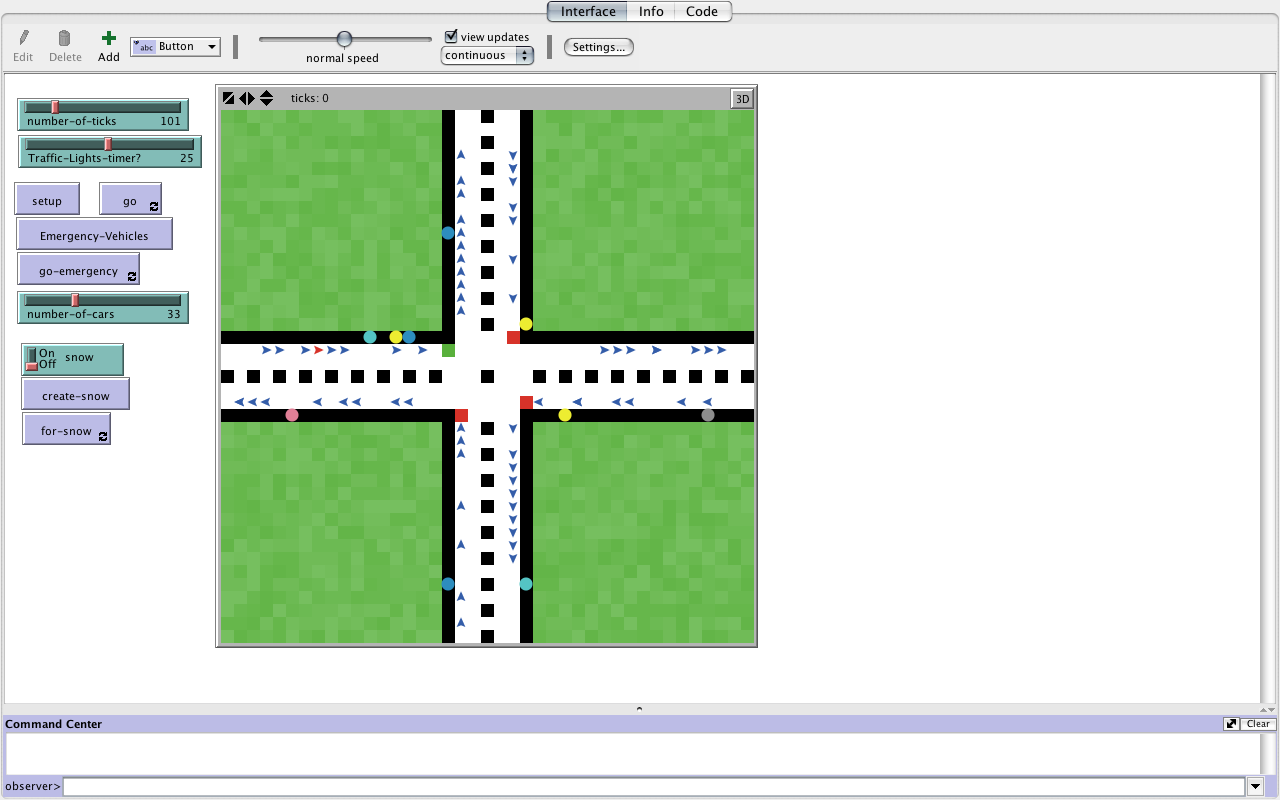
\includegraphics[width=0.9\textwidth]{ui.png}
\caption{\label{fig:ui}User Interface.}
\end{figure}
                                    
Now, user can start simulation by clicking setup button on the interface. We already uploaded a sequence diagram which depicts all the procedures which were initiated by the setup procedure.\newline
Among the procedures called by setup(), some of the most important methods are :

\subsubsection{\textbf{Draw-margins}}

This method is used to generate lanes along x-axis and y-axis in the NetLogo world. We categorize lane into eight types. In our project, Traffic simulator, in order to create road effect, we divided whole NetLogo world in such a way that some group of patches corresponds to a single lane. The patches corresponding to each lane are as follows: \newline
Lane0 - patches with  pxcor \(<\) -2 and (pycor = 2  or pycor = 1)\newline
Lane1 - patches with  pxcor \(<\) -2 and (pycor = -2 or pycor = -1)\newline
Lane2 - patches with pxcor \(>\) 2  and (pycor = 2  or pycor = 1)\newline
Lane3 - patches with pxcor \(>\) 2  and (pycor = -2 or pycor = -1)\newline
Lane4 - patches with (pxcor = 2  or pxcor = 1)  and pycor \(>\) 2\newline
Lane5 - patches with [ (pxcor = -2 or pxcor = -1) and pycor \(>\) 2\newline
Lane6 - patches with (pxcor = 2  or pxcor  = 1) and pycor \(<\) -2\newline
Lane7 - patches with (pxcor = -2 or pxcor = -1) and pycor \(<\) -2\newline
During simulation, the following are the lanes in NetLogo World

\begin{figure}[!ht]
\centering
\includegraphics[width=0.9\textwidth]{Design_of_Lanes_1.png}
\caption{\label{fig:dol1}Lanes.}
\end{figure}

\subsubsection{\textbf{Setup-cars}}

This procedure is responsible for creating turtles (which are treated as cars in our project ). This method in-turn instantiates another method namely “car-parameters” which assigns various parameters like speed, min-speed, max-speed. etc to all the cars. The following are calibrating parameters for vehicles in our project\newline
Maximum-speed : 90mph\newline
Minimum speed : 45mph\newline
Acceleration: 4m/(sec xsec)Deceleration : 8 m/ (sec x sec)\newline
While assigning various parameters to cars, we observed some random behaviour like turtles got undesirable xcor and ycor values, random heading. To overcome this unpredictable pattern we used some other code fragments namely

\begin{enumerate}
\item cars-only-in-lanes :
This part of code is used to make cars move on patches according to their lanes which is determined by the variable “lane”.\newline
\item assign-correct-coordinates:
when lanes turned into other lanes, this method makes sure to place them in the acceptable lanes as per their turn and this is decided by the variable “change-lane”.
\end{enumerate}

\subsubsection{\textbf{separate-cars}}

When creating cars for the first time, there is a chance of placing more than one turtle on one patch. If we allow this, it leads to serious problems as we don’t get desired behaviour because of more than one car at one place. To overcome this problem, we used “separate-cars” procedure.\newline 
This procedure will compel every turtle to verify whether there are any other turtles on the very same patch it presents. If present, the turtle will move forward one patch ahead. In this way, turtle moves forward until no other turtle is present on that location except itself.\newline
The code of this method is as follows:

\begin{figure}[!ht]
\centering
\includegraphics[width=0.8\textwidth]{separate_cars.png}
\caption{\label{fig:sc}Separate-Cars Code Snippet.}
\end{figure}

\subsubsection{\textbf{forward-cars-as-per-speed}}

After creating cars ( turtles ), it is very important to make them move similar to the real world vehicles on the roads. The code for this method is as follows:

\begin{figure}[!ht]
\centering
\includegraphics[width=0.8\textwidth]{forward_cars.png}
\caption{\label{fig:fcaps}Forward-Cars-As-Per-Speed Code Snippet.}
\end{figure}

This is done by code fragment “forward-cars-as-per-speed”. This procedure in turn uses two other small methods namely\newline
a)	accelerate-the-car : 
This code is implemented by the cars to accelerate themselves when there is no car ahead of them. Each car will know its front car by the variable “front-car”. The code for this method is as follows:

\begin{figure}[!ht]
\centering
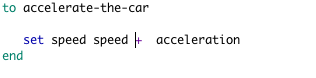
\includegraphics[width=0.6\textwidth]{accelerate.png}
\caption{\label{fig:a}Accelerate-the-Car.}
\end{figure}
                                  
b)	decelerate-the-car:
As the name of the method “decelerate-the-car” signifies, it decelerates the car if there is any other car infront of it thus achieving real life behavior of cars. The code for this is as follows :

\begin{figure}[!ht]
\centering
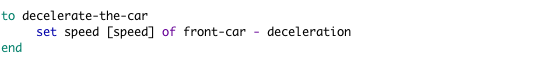
\includegraphics[width=0.8\textwidth]{decelerate.png}
\caption{\label{fig:d}Decelerate-the-Car.}
\end{figure}	

\subsubsection{\textbf{change-green-light-NW}}

As our problem here is a traffic simulator, traffic lights forms an integral part of the system. In our project, we have 4-lane junction. Therefore we considered traffic lights at four different positions namely
                     
\begin{enumerate}
\item North-west
\item North-east
\item South-east
\item South-west
\end{enumerate}
In NetLogo world, during simulation the traffic lights are placed at respective locations as shown in the figure.

\begin{figure}[!ht]
\centering
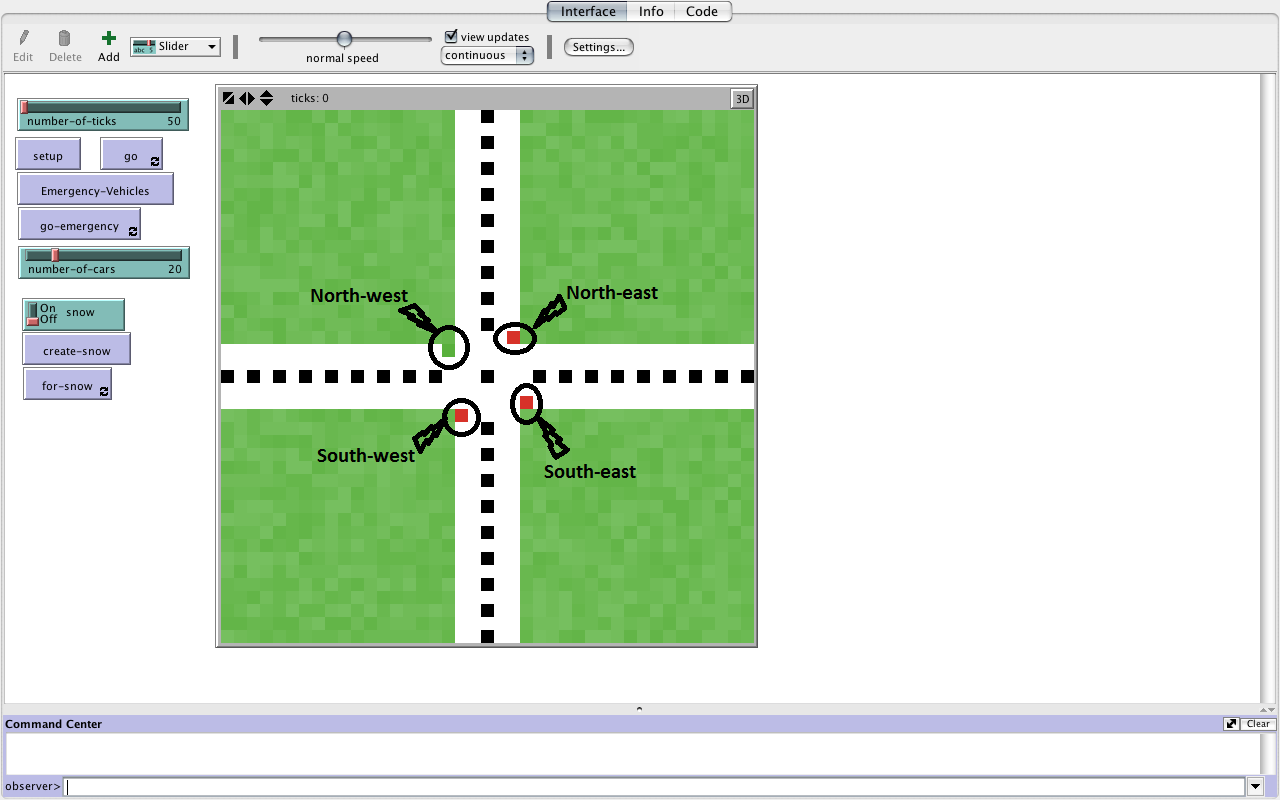
\includegraphics[width=0.8\textwidth]{tl.png}
\caption{\label{fig:tl}Traffic Lights.}
\end{figure}

Now, the code of the method “change-green-light-NW” is used to make North-west light as green and remaining as red. The code snippet for the above method is as follows:

\begin{figure}[!ht]
\centering
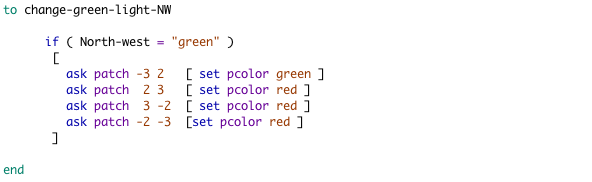
\includegraphics[width=0.8\textwidth]{tlcs.png}
\caption{\label{fig:tlcs}Changing Green Light Code Snippet.}
\end{figure}
                                       
 The other methods which follow the same pattern as above are 
\begin{itemize}
\item change-green-light-NE
\item change-green-light-SE
\item change-green-light-SW
\end{itemize}



\subsubsection{\textbf{go()}}

User can initiate “go” procedure by clicking go button on the interface tab. When one observers closely there is a small symbol on the bottom right side which clearly depicts that it is a forever button i. e. If you click this button once, all the methods which will be called by go procedure are instantiated repeatedly until you click it once again. ( In general, once you click any forever option enabled button, it will remain black signifying that it is running repeatedly and this can be clearly visible as the tick number goes on increasing. Once you click it again, it will turn normal and the method calling is stopped)\newline
The important methods that are being called by the go procedure are:


\subsubsection{\textbf{move()}}


This is one of the most trivial methods among all others. It is responsible for the movement of cars depending upon the traffic lights. For example, if North-east is green”, then all the vehicles in the lanes 0, 7, 3 should be static and vehicles in the lanes 1, 2, 5, 4, 6 can move according to their speeds. This is achieved by calling move method repetitively. This move method in turn call other methods namely\newline
\begin{enumerate}
\item move-cars()\newline
For example, if a vehicle moves from lane0 to lane2, then the lane variable associated with that vehicle should be updated from 0 to 2 because at the moment the vehicle is in lane2. This is very important issue to be addressed as we have coded our project entirely around dividing the whole NetLogo world into lanes. If this was not addressed, then we couldn’t have achieved any normal real life behavior like lane changing. The procedure “move-cars” is responsible for making vehicles following that behavior of updating of its lane variable depending upon the lane on which they stood.
A code snippet from move-cars method is as follows:

\begin{figure}[!ht]
\centering
\includegraphics[width=0.8\textwidth]{move_cars.png}
\caption{\label{fig:mc}Move Cars Code Snippet.}
\end{figure}

\item separate-cars2()\newline
When North-west is green, eventually North-east, South-east and South-west are red. Thus vehicles with lane variable equal to 4, 3, 7 should stop moving. In real life, when there is a red light at a junction, all the vehicles will stop in a row right before the red light thus following the traffic rules.\newline
Moreover, in our project we used microscopic level approach, in which vehicle-following forms one of the main criteria. This real life behaviour is achieved by cars calling “separate-cars2” method repetitively while they are moving on lanes.\newline 
This method uses another method namely “stop-at-the-red-light”, as the name suggests stops the vehicles at the red light. When cars call these methods “separate-cars2” and “stop-at-the-red-light”, the following behaviour can be observed during the simulation.\newline 
\end{enumerate}
                         
\begin{figure}[!ht]
\centering
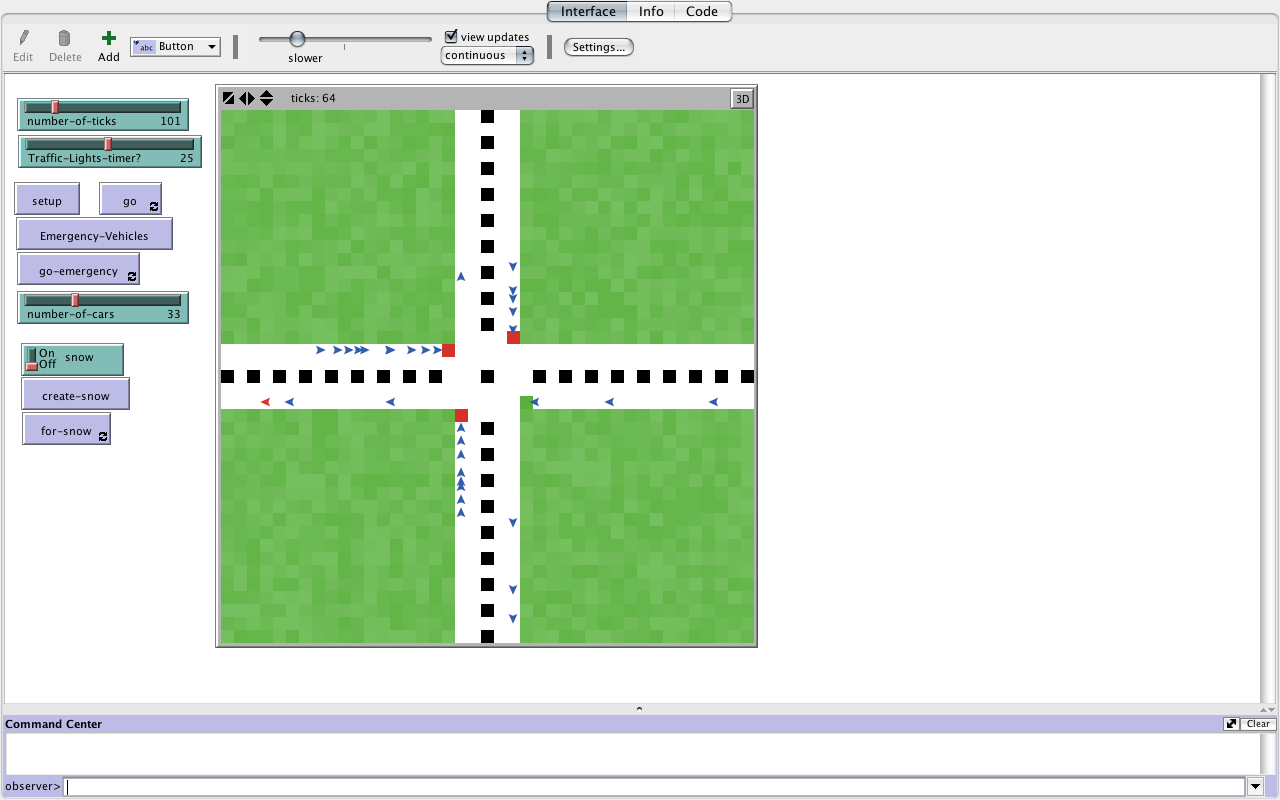
\includegraphics[width=0.8\textwidth]{sc2.png}
\caption{\label{fig:sc2}Separate-cars2 Code Snippet.}
\end{figure}

\subsubsection{\textbf{Change-globals-red()}}

The other important method that is employed by the go() procedure is “change-globlas-red()”. Showing traffic lights at the junctions is not itself address the problem of traffic simulation rather they should be changed periodically as in real life traffic light system. This is achieved as follows:\newline
On interface tab, we gave an option to select from a slider namely “Traffic-Lights-timer?”. This value is used as a parameter to change traffic lights systematically. For example, if user chooses 25 as the value for that slider, then for every 25 ticks traffic lights change from one color to another color. So, if at present the colors at\newline
                                     North-west = “red”\newline
                                     North-east = “red”\newline
                                     South-east = “green”\newline
                                     South-west = “red” and Traffic-Lights-timer? = 30 and tick = 260 ( let us assume it is  updated momentarily just now). Then, immediately when tick = 290, automatically the following changes will be observed in traffic light.\newline 
                                      North-west remains “red”\newline
                                      North-east remains “red”\newline
                                      South-east turns “red “\newline
                                      South-west turns “green “(Thus allowing lanes from lane7 to move).\newline
The above can be verified by the following diagrams

\begin{figure}[!ht]
\centering
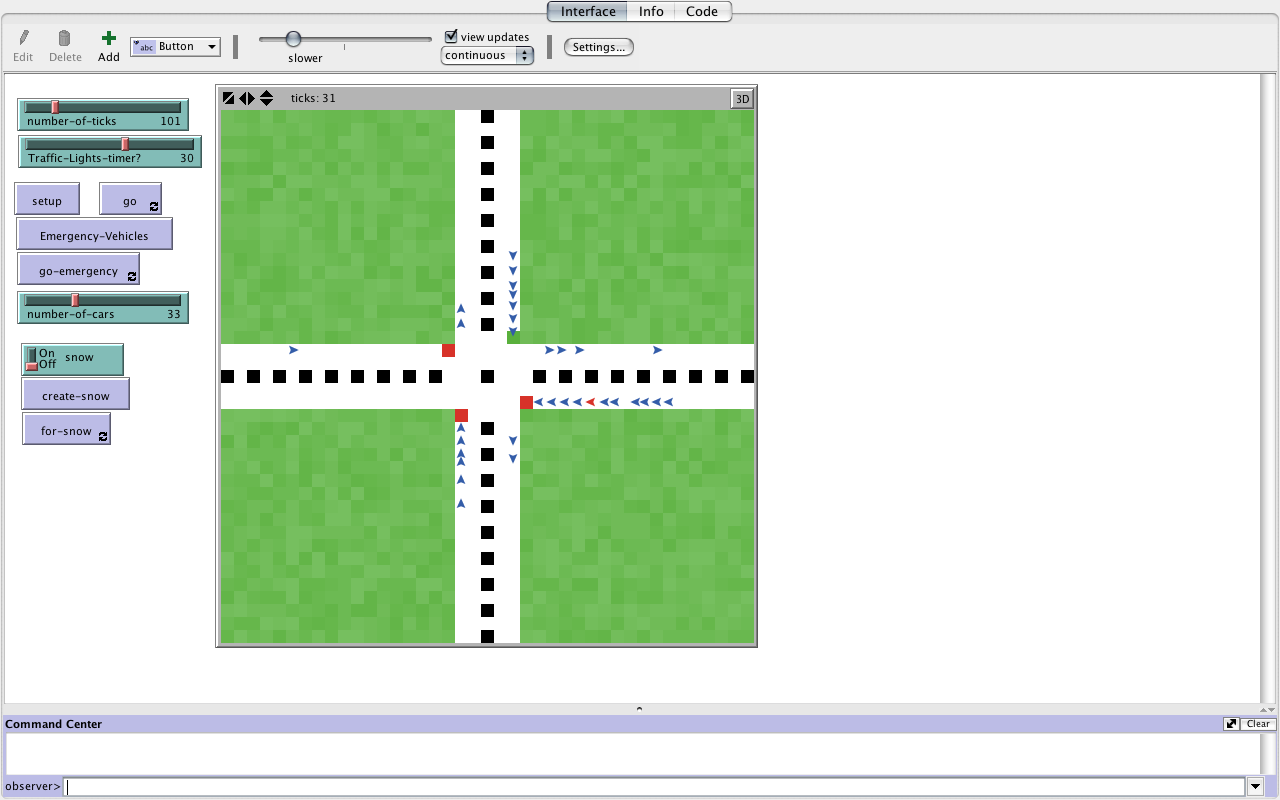
\includegraphics[width=1.0\textwidth]{neg.png}
\caption{\label{fig:neg}North-east-green.}
\end{figure}

\newpage

\begin{figure}[!ht]
\centering
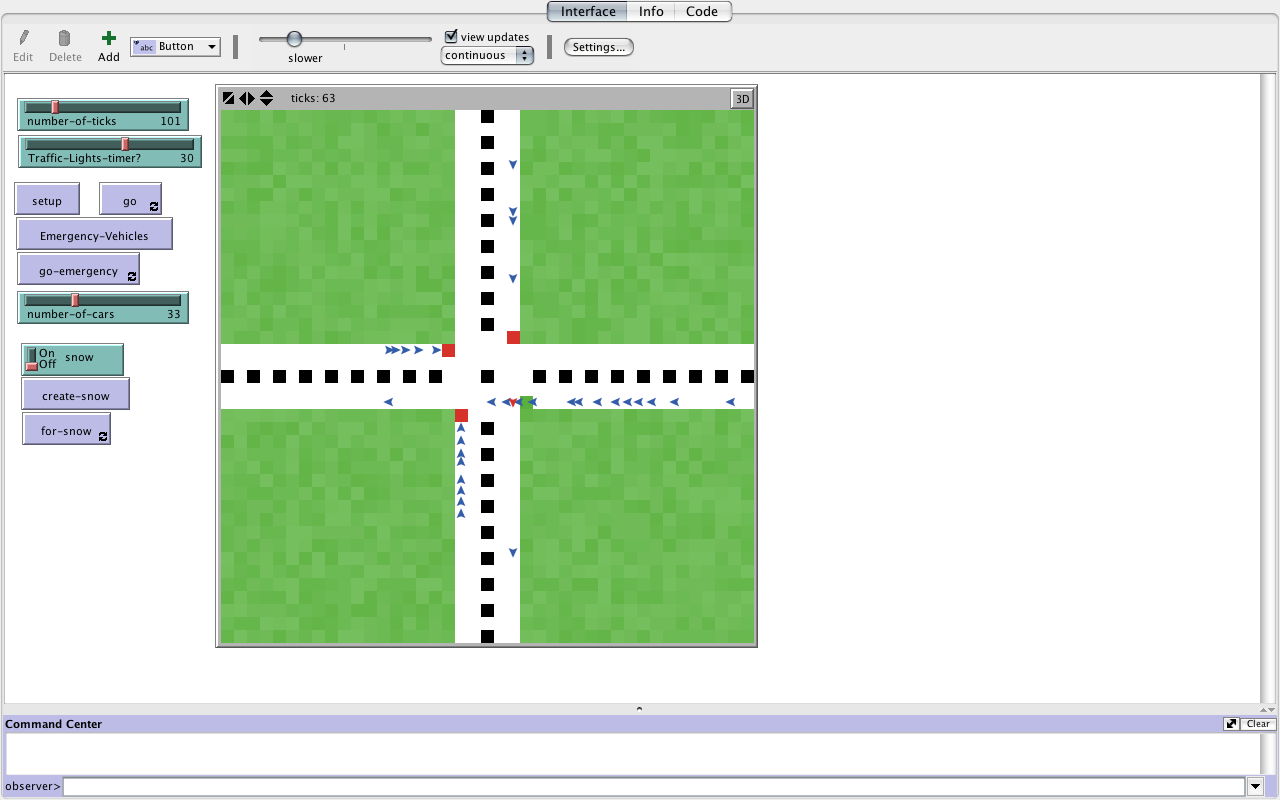
\includegraphics[width=1.0\textwidth]{seg.png}
\caption{\label{fig:seg}South-east-green.}
\end{figure}
                        
File Operations: \newline
In our project, one of the main requirement is to generate a report which collectively maintains all the data regarding the objects that are employed in simulation i. e. cars, pedestrians, emergency vehicles, etc. For this to be achieved we used to file procedures namely :
\begin{enumerate}
\item create-text-file
\item write-to-file
\end{enumerate}

\subsubsection{\textbf{create-text-file()}}
The code under this method is as follows:

\begin{figure}[!ht]
\centering
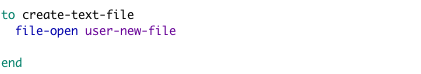
\includegraphics[width=0.9\textwidth]{ctf.png}
\caption{\label{fig:ctf}creat-text-file.}
\end{figure}

In this procedure, we use a command namely “file-open user-new-file” which will enable the user to create a text file and can save the file at his desired location. The following screen-shot explains this diagrammatically.
\newpage
\begin{figure}[!ht]
\centering
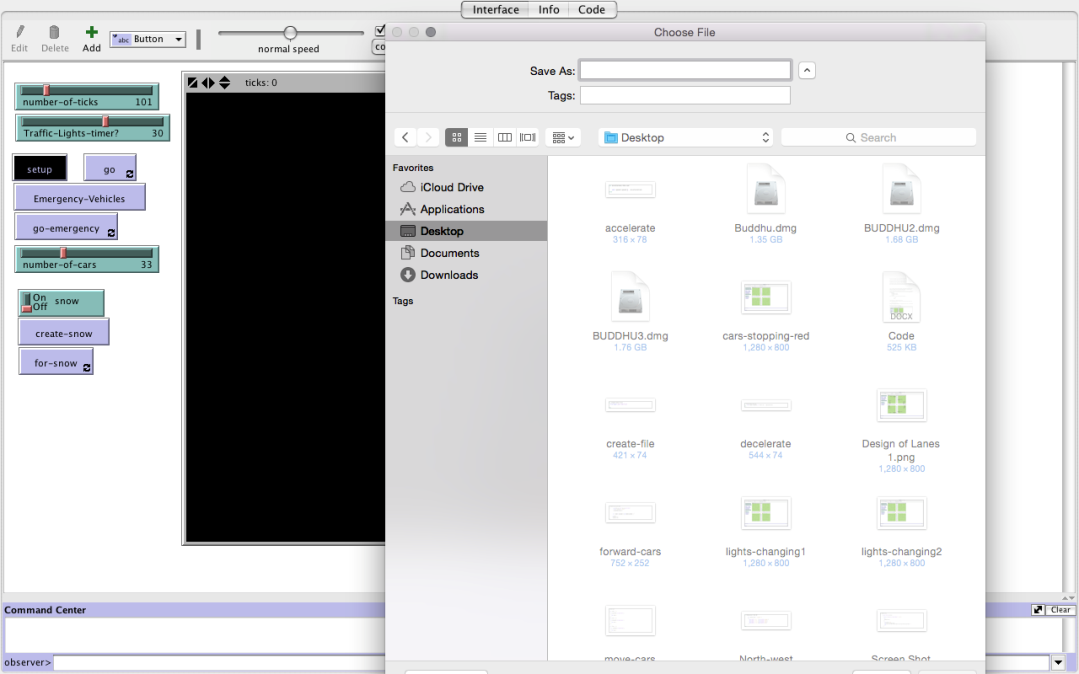
\includegraphics[width=0.9\textwidth]{cf.png}
\caption{\label{fig:cf}Creating file.}
\end{figure}

After creating a file, we have to enter data regarding the simulation for every tick. This is fulfilled by calling “write-to-file” method at the end of “go()” procedure. The code of this “write-to-file” is as follows:

\begin{figure}[!ht]
\centering
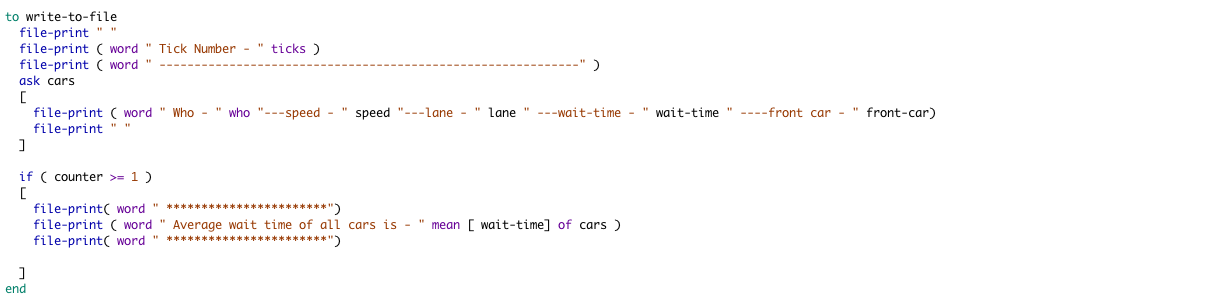
\includegraphics[width=1.5\textwidth]{wtf.png}
\caption{\label{fig:wtf}write-to-file.}
\end{figure}

\section{SOFTWARE TESTING}

Testing finishes an assortment of things, however in particular it quantifies the quality of the software an individual is developing. This perspective presupposes there are defects in the software holding up to be found and this perspective is once in a while disproved or debated upon.
\subsection{UNIT TESTING}

The primary goal of unit testing is to take the most minute piece of the testable software in the application, separate it from the remaining part of the code, and determine whether it behaves exactly as it is supposed to act. Each unit is tested separately before integrating it into the modules to test the interfaces between those modules. NetLogo ‘Test’ Extension lets one define and run unit tests for NetLogo code.\newline 
We ensured that the units worked manually. However, we didn’t have a proper unit test case coverage. Hence, it was carried out only for the selective important methods by the developers.

\subsection{FUNCTIONAL TESTING}

Functional testing is a testing process used within software development in which the software is tested to check if  it adheres to all the requirements. Functional testing is a good way of checking a particular software to check if it has all the required functionalities that is specified within all the functional requirements.\newline 
It was the responsibility of each team to ensure that the features to be released for the sprint were checked before its integration. It was also necessary to ensure that the feature did not slow down the existing functionalities.

\subsection{ERROR TESTING}

Tests will be completed to guarantee that each and every requirement is implemented accurately; these requirements will be ticked off as they are executed and tested. Different situations will be tested to guarantee that no blend of events can bring about an error at runtime. These tests will be continuous and will be determined as and when they occur, in this way they don't require unequivocal test plans. Some illustration test situations are:
\begin{itemize}
\item Running a simulation without any vehicles.
\item Running a simulation without any roads.
\item Attempt to create more number of vehicles than the number of roads.
\item Enter invalid inputs through sliders.
\end{itemize}

\subsection{TESTING ENVIRONMENT PROPERTIES}

OS: Windows 7 Home Premium\newline
Architecture: 64 bit\newline
Processor: Intel(R) Core(TM) i5-2450M\newline
CPU Processing Speed: 2.50 GHz\newline

\section{TEAM WORK}

\subsection{DIVISION OF TEAMS}

As mentioned earlier, we adopted the Agile Development Methodology for the development of our software. The group was divided into two sub teams namely the User Interface Team (Front End) and Simulation Team (Back End), with each of the team and its members focusing on one of the two major components at a high level of architecture. Each team then recognised their major tasks and sub-tasks to ensure cross team and parallel development. We followed a sprint model with regular status updates in each scrum meeting for the identification of tasks, allocation of tasks, development, testing, bug fixing and the documentation of each Sprint.

\subsection{WORK DIVISION}

The Agile Development approach was adopted. This helped the two teams, the User Interface Team and the Simulation Team to collaborate well among each other. During the meetings, the teams identified the tasks involved, divided the tasks among the group members and each member was assigned a role. The members of the team met twice every week to discuss important matters which could not be well explained over text messages, emails or phone calls.\newline
Members and their respective roles:
\begin{itemize}
\item Project Coordinator: Vikram Prabhu
\item Software Architect: Bhabishya Shrestha managed most of the tasks. Vijay Kumar, Praveen Allu, Nuruzzaman Shahin and Vikram Prabhu also contributed to the tasks.
\item Quality Tester: Nuruzzaman Shahin managed most of the testing phase. Vijay, Bhabishya, Vikram and Praveen also contributed to the testing phase.
\item User Interface Developers: Praveen Allu headed the User Interface Team. The other developers in the User Interface team were Bhabishya Shrestha and Nuruzzaman Shahin.
\item Simulation Developers: Vijay Kumar headed the Simulation Team. The other developer in the Simulation team was Vikram Prabhu.
\end{itemize}

\subsection{COLLABORATION TOOLS}
We used the following collaboration tools:
\begin{itemize}
\item Design and Architecture: ArgoUML
\item Project Management: Freedcamp 
\item Version Control: GitHub
\item Documentation Report: LateX
\item Means of communication: WhatsApp Messenger, Gmail, Outlook
\end{itemize}


\section{CRITICAL EVALUATION OF THE PROJECT}

\subsection{THE STRENGTHS}

\subsubsection{THE STRENGTHS IN CONCEPT}

Our product allows the user to model the road network very closely to the real-life traffic scenario and make high level infrastructure choices. 
For example:	
\begin{itemize}
\item User can model the diversity of vehicles driver behaviours and road/weather conditions.
\item Allowing a traffic engineer to test any traffic light configuration and their synchronisation at any point in the  simulation. This helps him engineer efficient traffic flow while ensuring safety.
\end{itemize}

The behaviour of the vehicles has been attained by maintaining minute variations in the behaviours of various drivers, which in-turn: 
\begin{itemize}
\item The desired speed of the vehicle.
\item The safe distance it keeps between other vehicles in front of it.
\end{itemize}


\subsubsection{THE STRENGTHS IN THE APPROACH CHOSEN}

Once we chose the approach, our group spent a large amount of time just considering various scenarios, drawing the UML diagrams and improving the concept before even starting a single line of code. After decomposing our system into its independent components and classes, we allocated the work amongst ourselves in a mature and non- conflicting way. This way, we avoided conflicts among the group members. It also prevented any repetition in code which would directly lead to wastage of efforts. This, along with a clear understanding of our skillset and matching responsibilities according to our strengths allowed us to successfully develop this project.

\subsection{THE WEAKNESSES}

Any piece of design and code of a software is unavoidable without errors and bugs due to time constraints which highly matters in this current project. We have addressed most of these issues during the different stages of the software development life cycle. But the following issues were identified but unable to address due to lack of time and resources:\newline
The scope of improvement for automated unit testing\newline
The source code entirely was intensively tested manually during all the stages of development and integration with the functional, integration and performance testing but it only failed to accomplish a sufficient level of automated unit testing coverage. This was done during the development stage.\newline
Scope of better allocation of resources and time for identified improvements\newline
At the start, the leading of the testing task was assigned to a member exclusively but during the course of the project development it was distributed amongst the whole group due to lack of the assigned member's involvement. A much better job could have been done by identifying the potential of the team and allocating the time and resources to enhance the areas we all were lacking in.

\section{FUTURE SCOPE}

\begin{itemize}
\item User Interface enhancements with appealing road network design and simulation. 
\item Roads with more than two lanes.
\item The Undo and Redo functionality for road network design and configuration. 
\item Implementing 3 Dimensional road networks which include bridges. 
\item Destination based routing for more than one destination. 
\end{itemize}

\section{PEER ASSESSMENT}
We agreed to equally split the 100 points amongst the five group members. This was be done without the knowledge of the other group members where in each member allocated their points to the other group members based on their performance and contribution to the project. Each member had a total of twenty points which was allocated to the other four members of the group excluding himself.\newline
We agreed to use this method of assessment as this was an unbiased method. There was a slight problem when it came to the two teams -- User Interface Team and the Simulation Team as the members of one team did not know the contribution and performances of the members in the other team. Hence, we then came to a conclusion that each member of the KingsMen Group would contribute to each and every task and that’s when assigning the number of points to each member became easier.
\subsection{Handling the Team Conflict}
Conflicts arise even amongst the best of friends. All the conflicts that arose in the KingsMen Group was handled in a matured manner without creating a fuss about anything at all even in the absence of a member during the group meetings. The same was followed even in the accomplishment of deadlines for particular tasks.
\begin{itemize}
\item If any member was absent for any group meeting, it was the sole responsibility of the member to update himself by checking FreedCamp and also his emails to see what he had missed out and also to check if any task was assigned to him with its corresponding deadline.
\item There were times during the meetings or discussions when there was a difference of opinion among the members of the group. An unbiased opinion was taken into consideration. The most beneficial option for the project was then agreed upon.
\item If a particular member failed to meet any of the task deadlines, it was dealt with high priority.
\end{itemize}

We assigned the following points to each member \newline

\begin{tabular}{|c|c|}
	\hline
	\textbf{Member Name} & \textbf{Points Allocated}\\
    \hline
    Vikram Prabhu & 20\\
    \hline
	Vijay Kumar Badatala & 20\\
    \hline
    Praveen Allu & 20\\
    \hline
    Bhabishya Shrestha & 20\\
    \hline
    Nuruzzaman Shahin & 20\\
    \hline    
\end{tabular}

\section{BIBLIOGRAPHY}

\begin{enumerate}

\item NetLogo User Manual: http://ccl.northwestern.edu/netlogo/docs/

\item Wilensky, U. (1998). NetLogo Traffic 2 Lanes model.\newline
http://ccl.northwestern.edu/netlogo/models/Traffic2Lanes. Center for Connected Learning and Computer-Based Modeling, Northwestern University, Evanston, IL

\item North, M.J., and Burkhart, R.M. (2002). Agent-Based Methods, Toolkits, and Techniques. In M. J. North, C. M. and D. L. Sallach (Eds.), Proceedings of the Agent 2002 Conference on Complex Interaction and Social Emergence (pp. 3-10). IL: Argonne National Laboratory and University of Chicago

\item Tisue, S., and Wilensky, U. (2004). NetLogo: Design and Implementation of a Multi-Agent Modeling Environment. Paper presented at the Agent2004 Conference, Chicago, IL
Steven F. Railsback; Volker Grimm (2011). \textit{Agent-Based and Individual-Based Modeling: A Practical Introduction.} Cambridge: Princeton University Press. ISBN 978-0-691-13674-5

\item Uri Wilensky; William Rand (2015). \textit{An introduction to agent-based modeling: Modeling natural, social and engineered complex systems with NetLogo.} Cambridge: MIT Press. ISBN 978-0-262-73189-8.

\item José M. Vidal (2010). \textit{Fundamentals of Multiagent Systems Using NetLogo}

\item TOMAS, V.R. and GARCIA, L.A., 2005. A cooperative multiagent system for traffic management and control, \textit{AAMAS '05: Proceedings of the fourth international joint conference on Autonomous agents and multiagent systems}, 2005, ACM Press pp52-59

\end{enumerate}

\section{APPENDICES}

\subsection{GITLOG}
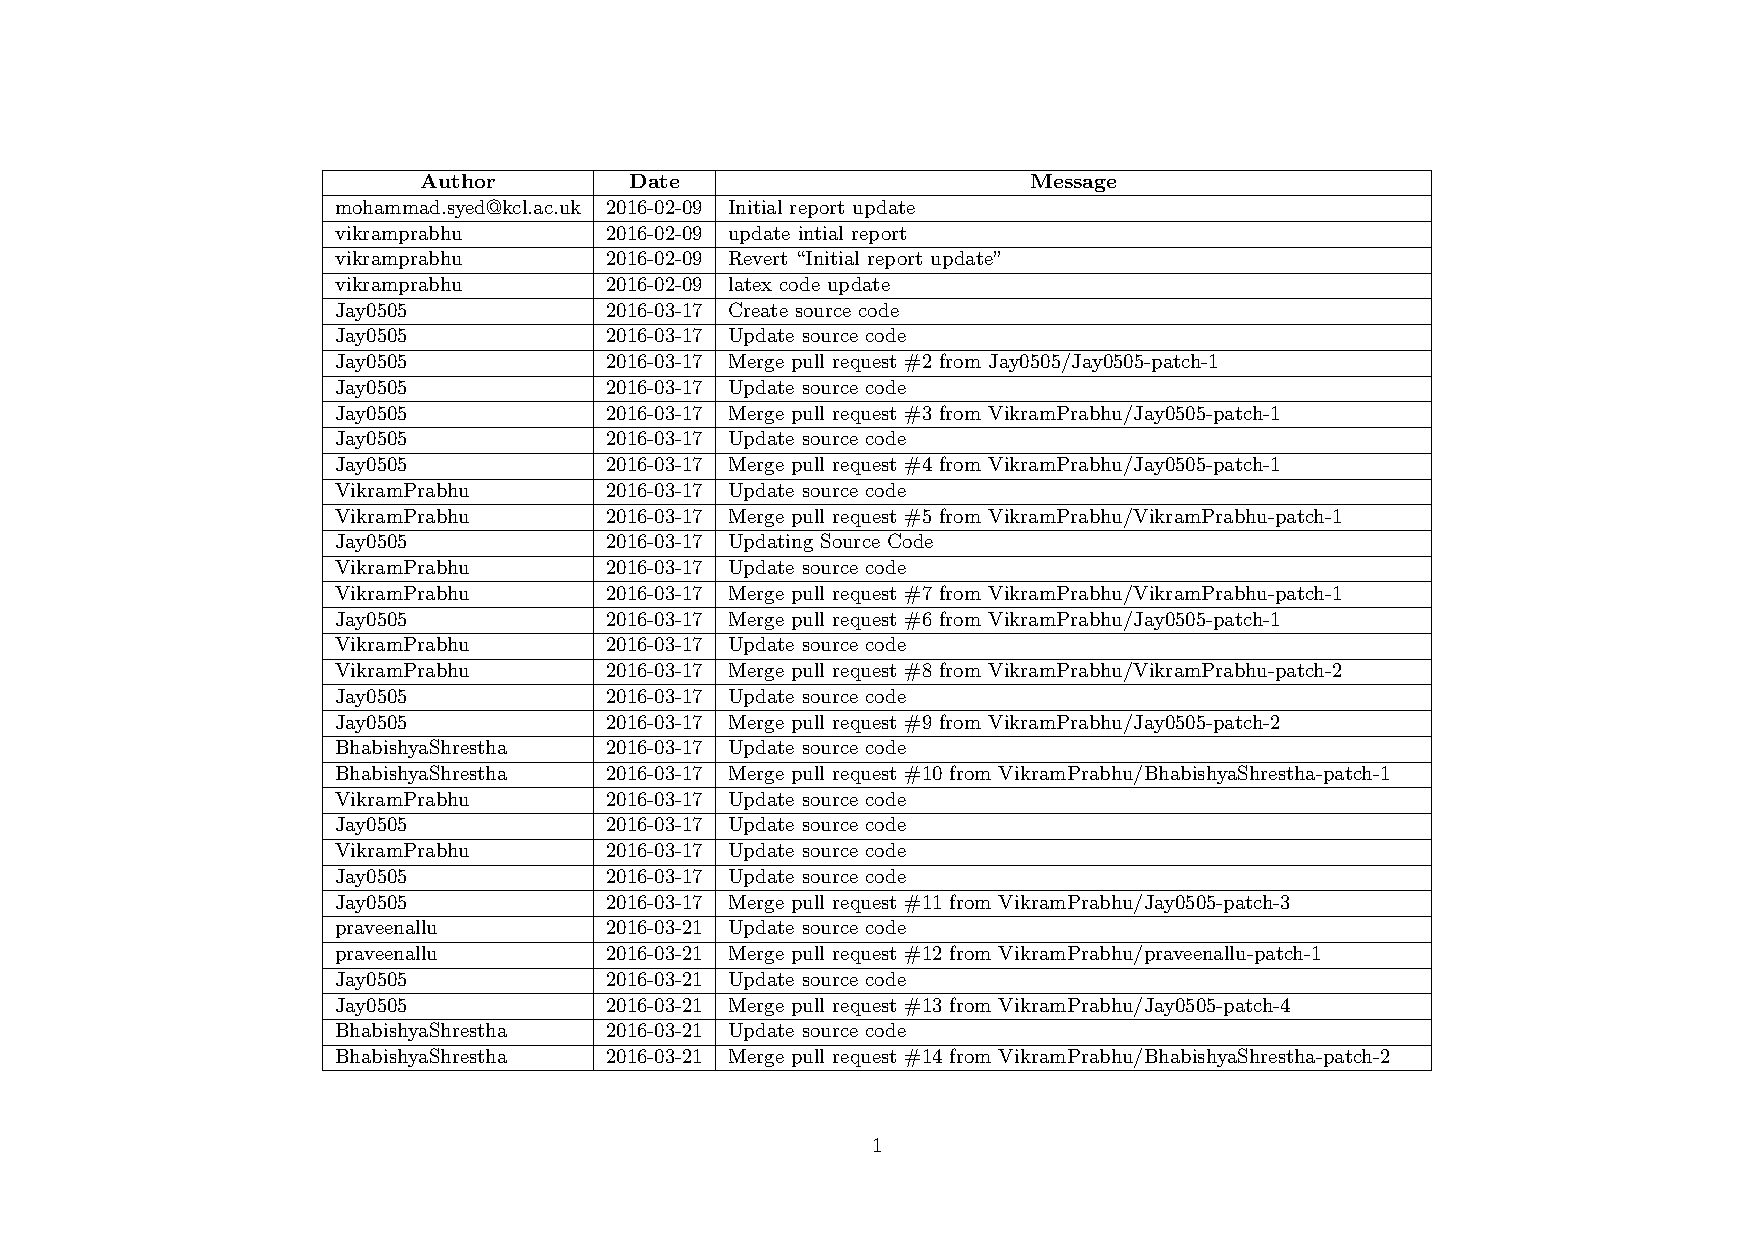
\includepdf[pages={1-5}]{gitlog.pdf}

\subsection{SOURCE CODE}
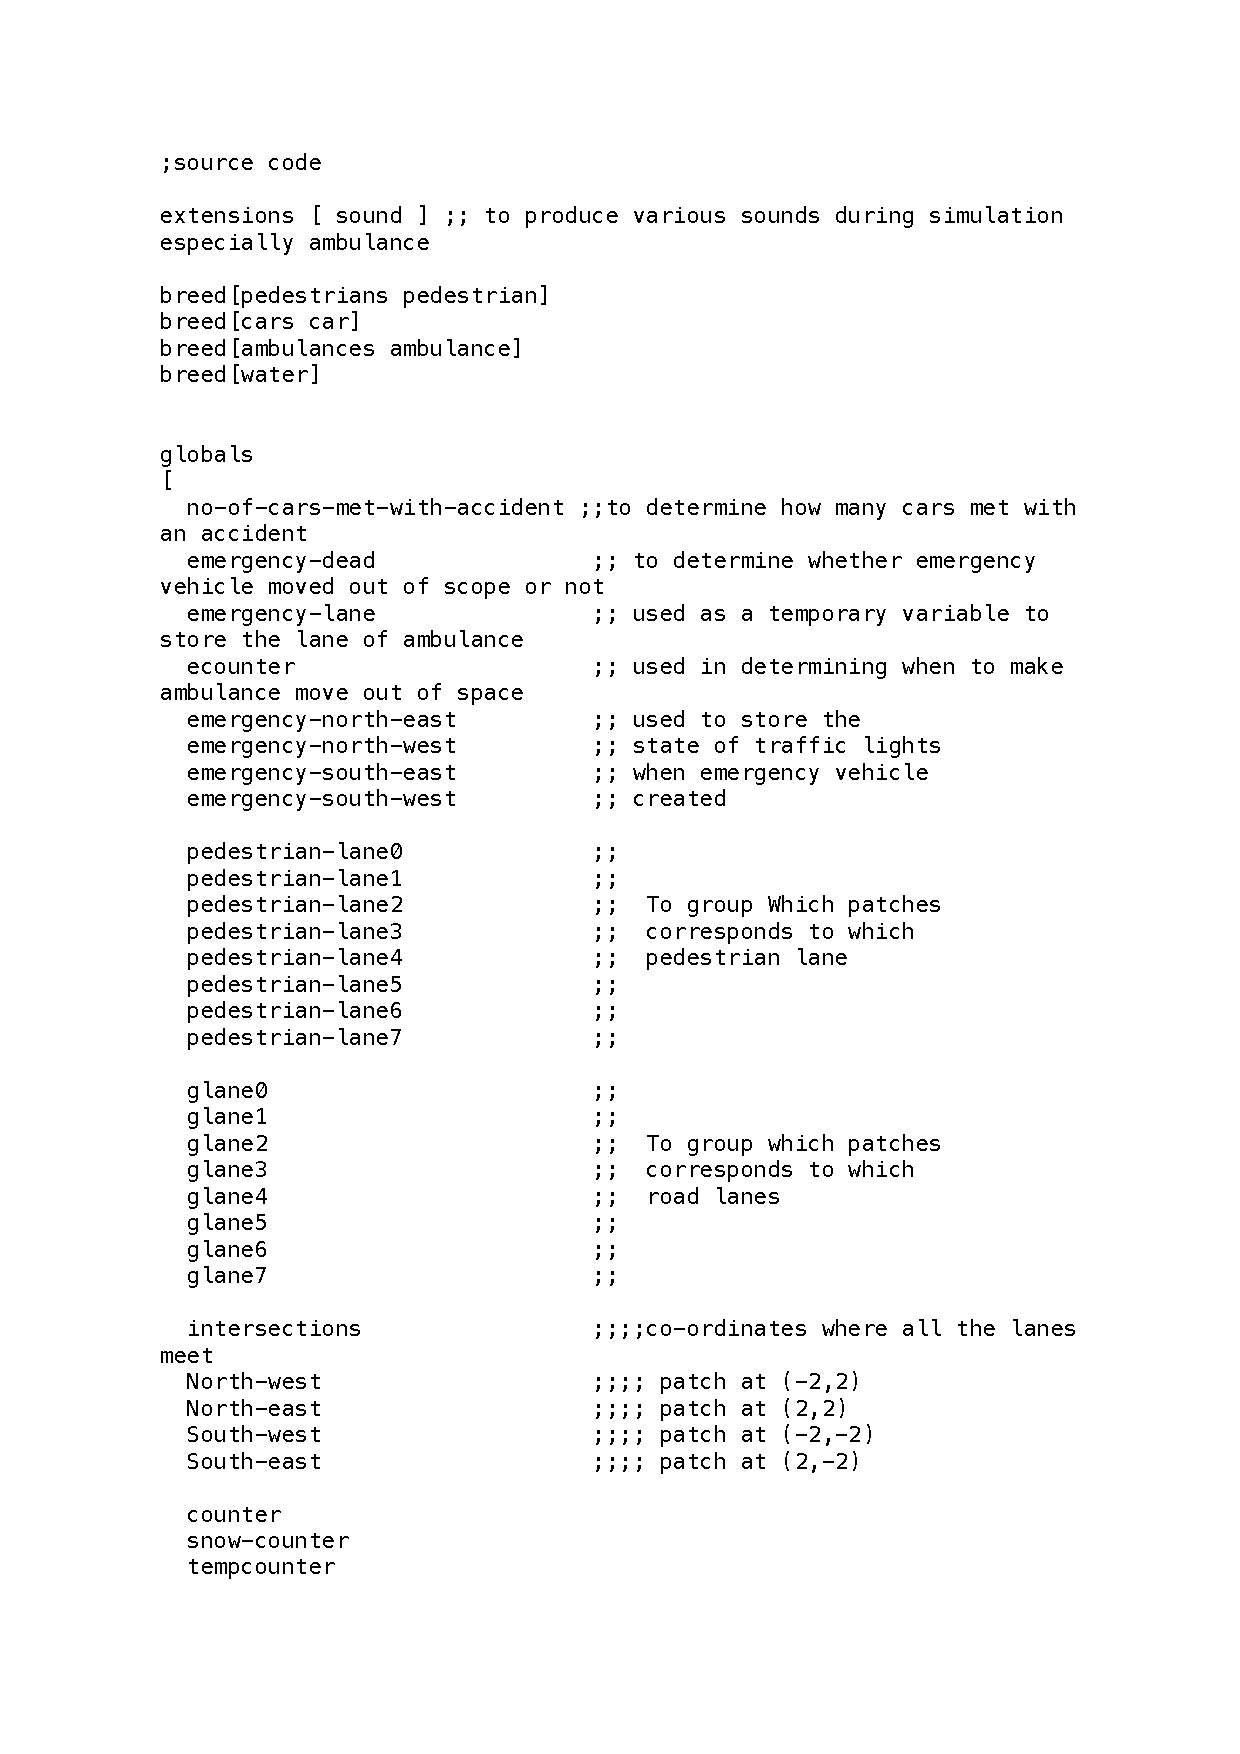
\includepdf[pages={1-51}]{sourcecode.pdf}

\end{document}